\section{Software Design}\label{sec:design}
\phantomsection

\subsection{UML Modeling}
The following chapter presents the system modeled in UML language. It contains the main diagrams that are necessary to document and understand the structure and behavior of the system. Before starting any real work, it is essential to define use case diagrams. 

Figure \ref{fig:umlusecase} contains the use case diagram related to the end-user application. This is a high level overview of main features available to users. Respectively, users will be able to access settings, statistics and sleep screen. In settings the user is given the option to set regular sleep time, which includes setting up the start, end of sleep and the days of the week when the user wishes to make the recording. The results of the recording are shown in statistics, which can be erased. Most important screen is the so-called ``sleep'' screen, where from the recording is being started and ended.

\begin{figure}[!ht]
\centering
  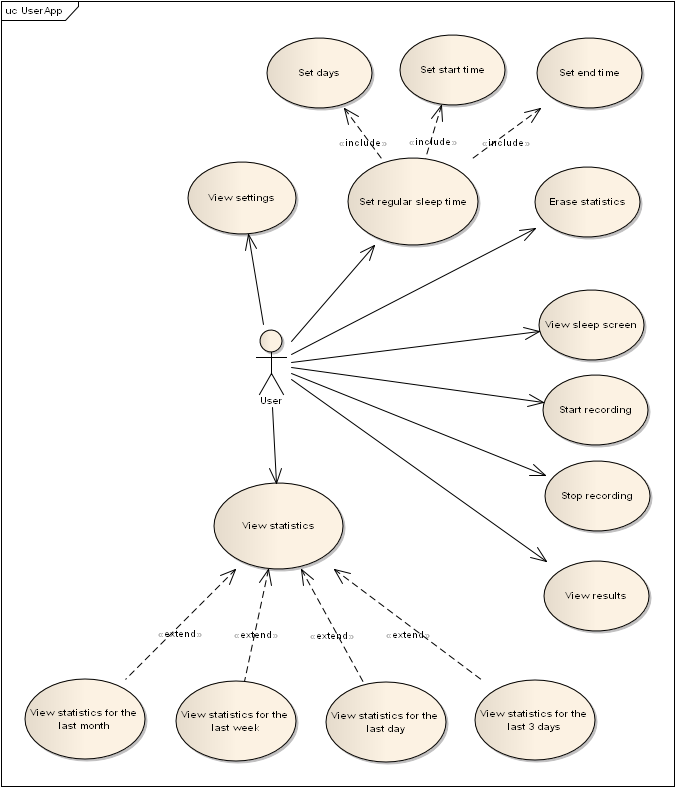
\includegraphics[width=12cm]{uml_usecase.png}
\caption{User application use case diagram}
\label{fig:umlusecase}
\end{figure}

To get a better idea of how the system works, several sequence diagrams are developed. A crucial part of the system is the digital signal processing. In the training phase the DSP is triggered by a worker which analyses data from Prague Psychiatric Center. 

In figure \ref{fig:umldsp} at first the worker establishes a connection to the training database and create features table, which is empty at the moment. Afterwards the worker loops over a set of signals stored as WAV data. The signal object reads the data by extracting the sampling rate and the data itself. The following signal is being slitted into smaller chunks to be filtered and extracted features from. The filtering part includes a low-pass filter, normalization, autocorrelation, computing power spectral density. By having the signal in its frequency domain a set of features are being extracted: local maximas from specially identified bins and regular size bin areas. The extracted features are stored in the table. Eventually after storing all the necessary data, the connection to the database is closed.

\begin{figure}[!ht]
\centering
  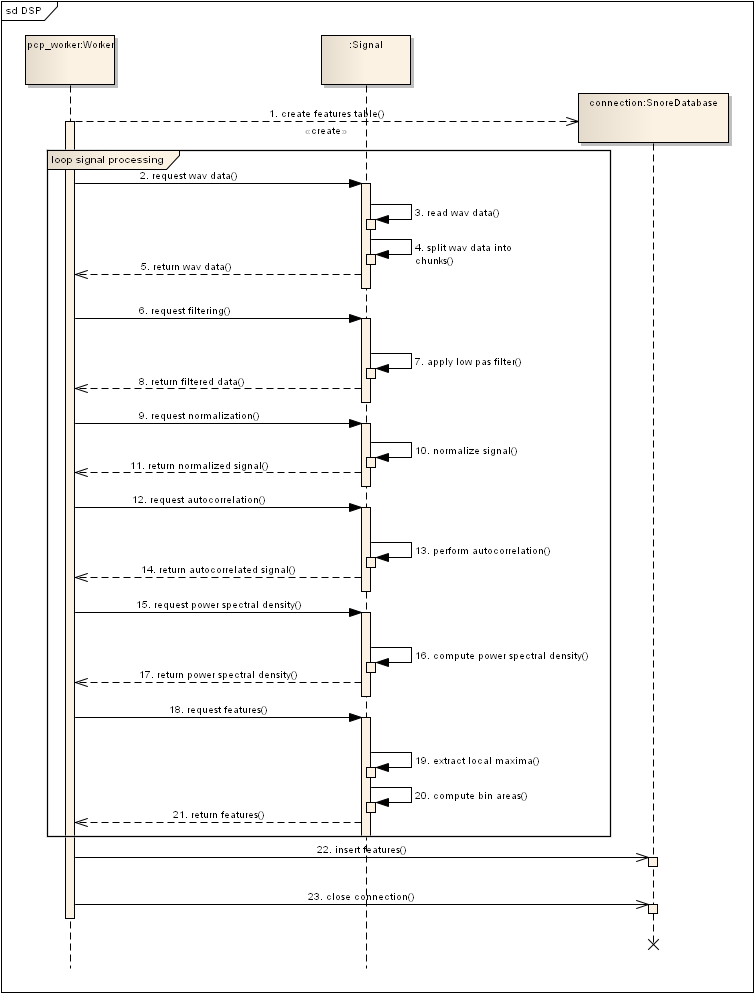
\includegraphics[width=15cm]{uml_dsp.png}
\caption{Digital signal processing sequence diagram}
\label{fig:umldsp}
\end{figure}

Considering that all the feature data is available and stored safely in the database, next step is the training stage represented in figure \ref{fig:umltraining}. The training worker will establish the connection to the ``snore'' training database, will select features and close the connection immediately after. 

The features will serve as training data to the Logistic Regression algorithm. Therefore the model will fit the samples and create a set of coefficients, that can be used in future predictions. Even though the fitting can happen on every requested prediction, it is inefficient. Hence the model object is deserialized into a JSON file, by storing prediction classes and the coefficients. After the state of the model is saved, the file handler is returned and the file is being closed. 

\begin{figure}[!ht]
\centering
  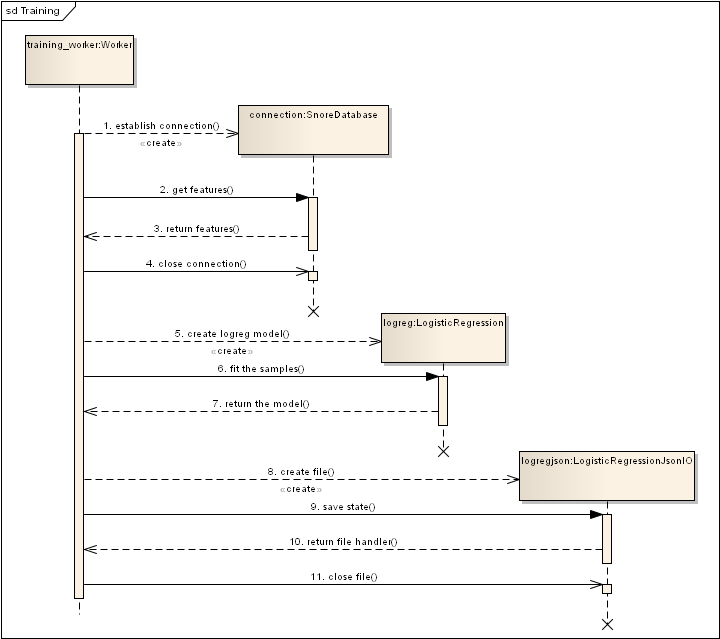
\includegraphics[width=15cm]{uml_training.png}
\caption{Training model sequence diagram}
\label{fig:umltraining}
\end{figure}

Figures \ref{fig:umldsp} and \ref{fig:umltraining} were dealing with the back-end functionality hidden to the end user. Conversely figure \ref{fig:umluserapp} presents the interactions of the user and the application. As soon as the user starts the application, he or she can see the main ``sleep'' screen where from the recording can be started. User sends the message asynchronously and can end the recording also asynchronously. The application receives the messages, stop the recording and starts processing the captured sound signal. 

The processing encapsulates the filtering of the signal and feature extraction. Each chuck of the signal will generate a set of features that will be inserted in a prediction database. 

\begin{figure}[!ht]
\centering
  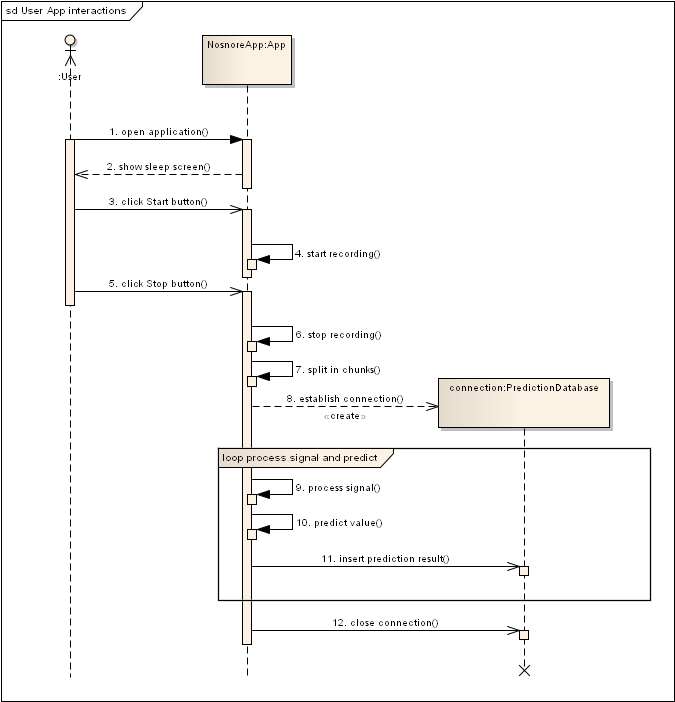
\includegraphics[width=15cm]{uml_userapp_interactions.png}
\caption{User application interactions sequence diagram}
\label{fig:umluserapp}
\end{figure}

Sequence diagrams were dealing with storing some data, thus it is necessary to create helper classes to deal with storage. Figure \ref{fig:umljson} contains a representation of classes used for JSON storage. The base class encapsulated the behavior of loading and dumping JSON from and into a file. The following functionality is being reused by classes that extend the basic functionality with some specific tasks. ``LogisticRegressionJsonIO'' class holds a pointer to the JsonIO class and offers the functionality to save and retrieve the state of the model.

Another similar paradigm is used for database storage in figure \ref{uml:umlsqlite}. For training purposes the most lightweight database is being used -- Sqlite. The base class encapsulates the connection object and the cursor object. Its methods can execute an SQL query or execute many queries simultaneously. Fetching of data can be accomplished using different types -- fetch all, fetch just one or fetch many. SqliteDatabase class creates the connection in its initializer and closes the connection by calling the ``close'' method explicitly.

The SqliteDatabase object can become a composite part of other derived classes. For instance SnoreDatabase which is used for storing training data adds methods for creating the features table, fetching the features from the database and inserting features. Similar functionality is added to the PredictionDatabase, which handles the new unlabeled features extracted from recorded signals.

\begin{figure}[!ht]
\centering
  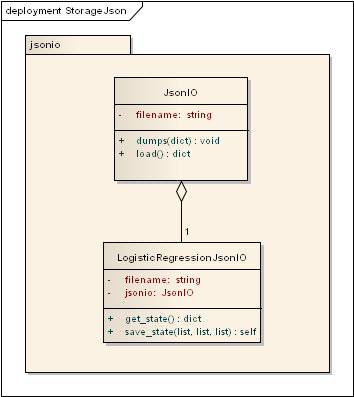
\includegraphics[width=8cm]{uml_class_json.png}
\caption{Json storage class diagram}
\label{fig:umljson}
\end{figure}

\vspace{5mm}

\begin{figure}[!ht]
\centering
  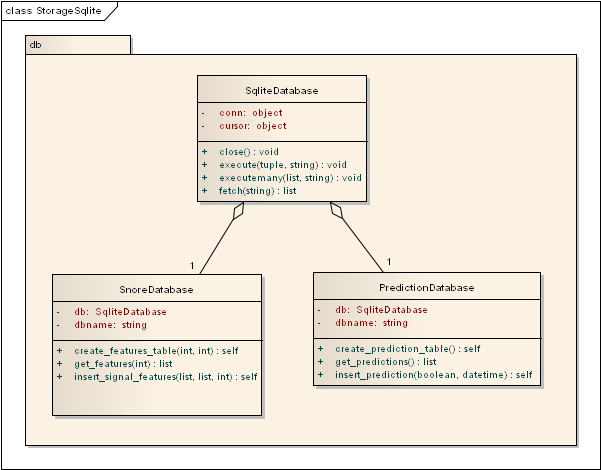
\includegraphics[width=13cm]{uml_class_sqlite.png}
\caption{Sqlite database storage class diagram}
\label{fig:umlsqlite}
\end{figure}

From the end-user application, it is important to present the screen management of the application. The Screen class presented in figure \ref{fig:umlscreens} is the generic class offered by the Kivy framework. It presents a public interface, which displays the public properties of the class. Three screen defined by the developer derive from Screen class, each having a different set of properties and functionality. For instance, the Sleep Screen contains a recorder object. 

The screens are being composite elements of Screen Manager, which keeps track of all screens and the current active screen. Aggregation relation is being used, because the screens are being destroyed in case the screen manager is destroyed. Same holds for the relationship between the application object and the screen manager.

\begin{figure}[!ht]
\centering
  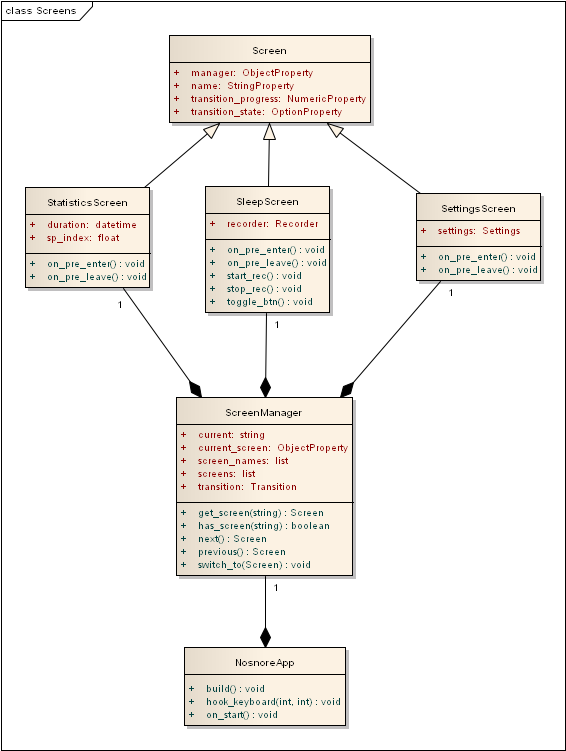
\includegraphics[width=13cm]{uml_class_screens.png}
\caption{Application screens class diagram}
\label{fig:umlscreens}
\end{figure}

A closer look at the Sleep Screen and Recorder classes is taken in figure \ref{fig:umlrecorder}. Recorder is a composite part of the Sleep Screen. The Recorder class itself is merely a facade to real recorders. The reason to create an extra level of abstraction is because the application is planned to be cross-platform software. Even though the looks, transitions and many other functions can be cross-platform, the capturing of sound is highly platform dependent. Therefore the Recorder class is dispatching the recording function depending on the platform. With this configuration it is easy to add new platforms. The ones defined here are DesktopRecorder and AndroidPlatform. One more element is present and it is the Processor that encapsulated the processing and prediction of the snore/nosnore classification.

\begin{figure}[!ht]
\centering
  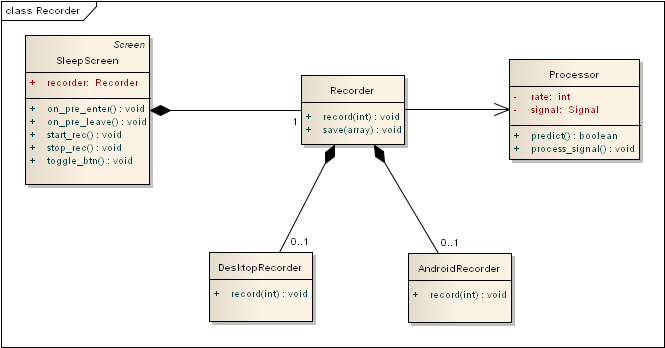
\includegraphics[width=15cm]{uml_class_recorder.png}
\caption{Recorder class diagram}
\label{fig:umlrecorder}
\end{figure}

The application has a bunch of states showed in figure \ref{fig:umlstate}. The initial state represents the start of the application. From the following state the user can transit to visualization of statistics, settings or start the recording. Stopping of the recording is only possible passing through the start of the recording. From all those states the user can exit the application, except for the ``Start recording'' state.

\begin{figure}[!ht]
\centering
  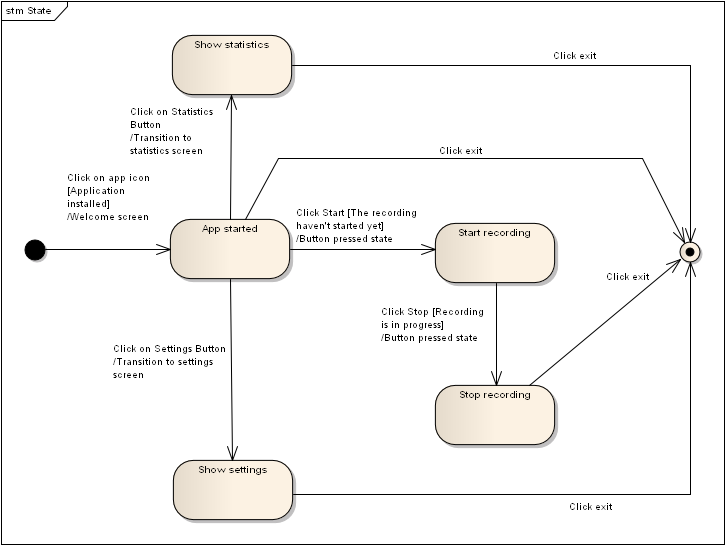
\includegraphics[width=15cm]{uml_state.png}
\caption{App navigation state diagram}
\label{fig:umlstate}
\end{figure}

Not much have been said about statistics, therefore figure \ref{fig:umlactivity} presents an activity diagram for statistics. On statistics screen user can select a period of time to visualize data. In case it represents a single day, than a screen with text will be shown with data about length of recording, length of snoring and possible chance of having Sleep Apnea. Otherwise a graph will be drawn with entries equal to the number of days selected. The bar chart shows the time of sleeping versus time of snoring. The activity diagram also has the possibility to clear all the statistics.

\begin{figure}[!ht]
\centering
  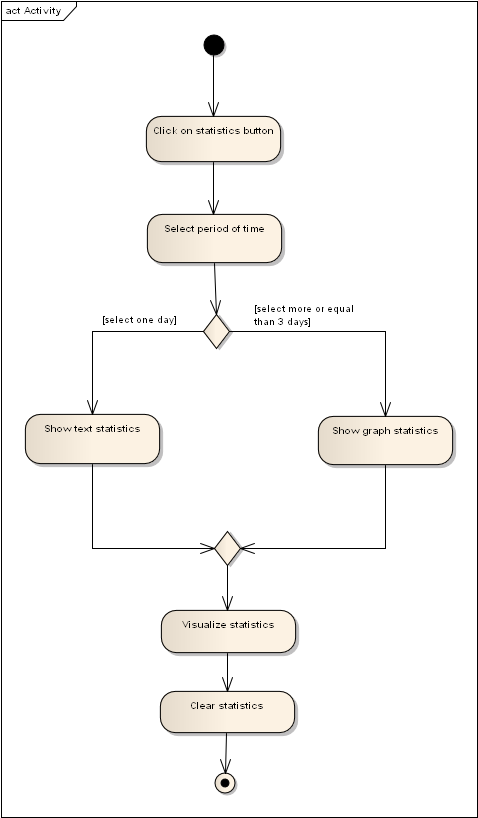
\includegraphics[width=10cm]{uml_activity.png}
\caption{Statistics activity diagram}
\label{fig:umlactivity}
\end{figure}

Components diagram in figure \ref{fig:umlcomponents} is very important for the following project, since it relies on a variety of free and open-source libraries and frameworks. The essential environment for development was Anaconda -- scientific Python distribution that consists of a set of popular scientific libraries like Numpy, Scipy, Sklearn, Matplotlib, Pylab. The core module is developed by the programmer and has modules for DSP processing, plotting and signals. The application is also dependent on tables that store important data. Actually the main dependency represents the Kivy framework -- open source Python library for rapid development of applications that make use of innovative user interfaces, such as multi-touch apps.

\begin{figure}[!ht]
\centering
  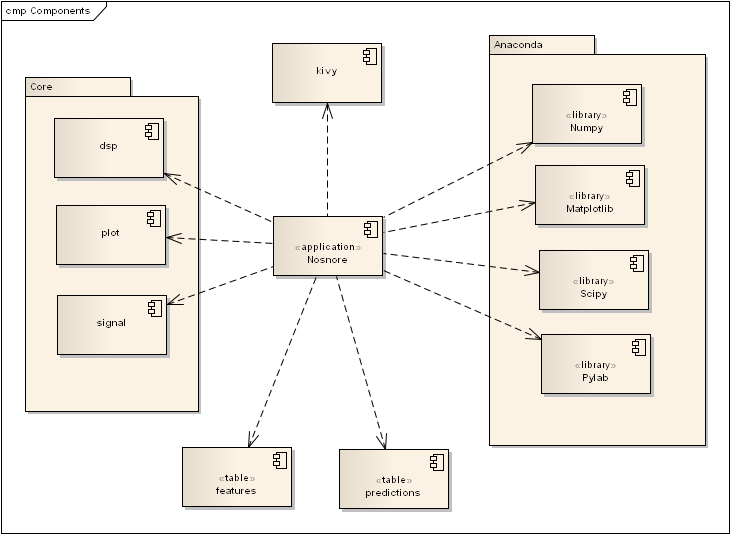
\includegraphics[width=15cm]{uml_components.png}
\caption{Application component diagram}
\label{fig:umlcomponents}
\end{figure}

The deployment diagram is missing, since this is a client-side application, which doesn't depend on Internet or communication with a remote server. This concludes the UML part of the project, that aimed at presenting the most relevant aspect of the system and covering the general architecture of the application.

\clearpage
